% Graphics for slide 6, in the order the PDF draws them.
\begin{tikzpicture}[remember picture, overlay, x=1bp, y=-1bp,
  shift={(current page.north west)}]
\path[fill=cFFFFFF] (0,0) rectangle (960,540);
\node[anchor=north west, inner sep=0pt] at (56.69,477.21) {
\includegraphics[width=73.42bp, height=37.42bp]{figures/fundamentals-of-hpc/p03-1.png}};
\path[fill=cEE7628,even odd rule] (57.18,55.73) ..controls(57.96,55.73)and(58.6,56.37)..(58.6,57.15) --(58.6,85.5) ..controls(58.6,86.28)and(57.96,86.91)..(57.18,86.91) ..controls(56.4,86.91)and(55.76,86.28)..(55.76,85.5) --(55.76,57.15) ..controls(55.76,56.37)and(56.4,55.73)..(57.18,55.73);
\node[anchor=north west, inner sep=0pt] at (420.53,86.91) {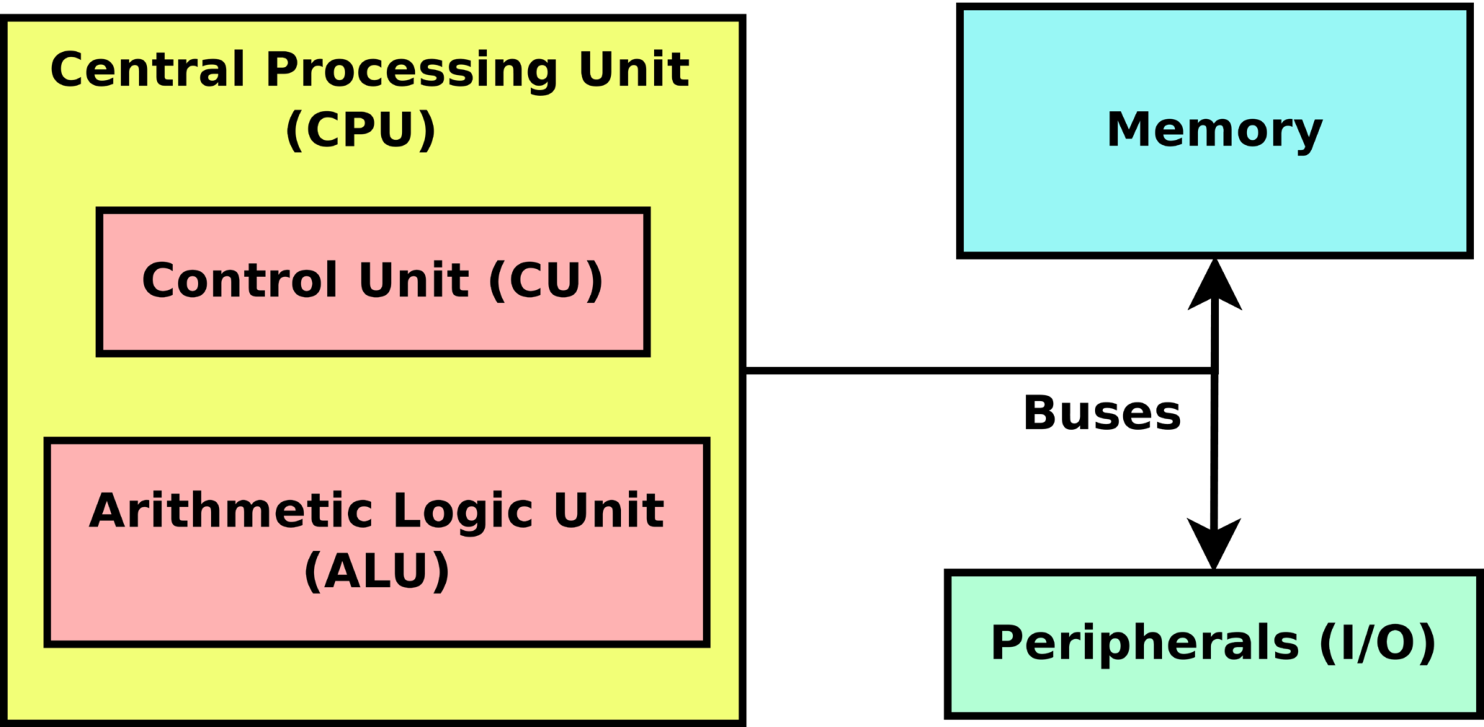
\includegraphics[width=494.32bp, height=241.87bp]{figures/fundamentals-of-hpc/p06-2.png}};
\path[fill=c2CA055,even odd rule] (56.69,383.95) ..controls(56.69,376.31)and(62.88,370.12)..(70.52,370.12) --(901.02,370.12) ..controls(908.66,370.12)and(914.85,376.31)..(914.85,383.95) --(914.85,439.26) ..controls(914.85,446.9)and(908.66,453.09)..(901.02,453.09) --(70.52,453.09) ..controls(62.88,453.09)and(56.69,446.9)..(56.69,439.26) --(56.69,383.95);
\end{tikzpicture}
